%%%%%%%%%%%%%%%%%%%%%%%%%%%%%%%%%%%%%%%%%
% Structured General Purpose Assignment
% LaTeX Template
%
% This template has been downloaded from:
% http://www.latextemplates.com
%
% Original author:
% Ted Pavlic (http://www.tedpavlic.com)
%
% Note:
% The \lipsum[#] commands throughout this template generate dummy text
% to fill the template out. These commands should all be removed when 
% writing assignment content.
%
%%%%%%%%%%%%%%%%%%%%%%%%%%%%%%%%%%%%%%%%%

%------------------------------------------------------------------------------------
%	PACKAGES AND OTHER DOCUMENT CONFIGURATIONS
%------------------------------------------------------------------------------------

\documentclass{article}

\usepackage{fancyhdr} % Required for custom headers
\usepackage{lastpage} % Required to determine the last page for the footer
\usepackage{extramarks} % Required for headers and footers
\usepackage{graphicx} % Required to insert images
\usepackage{lipsum} % Used for inserting dummy 'Lorem ipsum' text into the template
\usepackage{tikz}
\usepackage{tikzscale}
\usetikzlibrary{automata,positioning}
% Margins
\topmargin=-0.45in
\evensidemargin=0in
\oddsidemargin=0in
\textwidth=6.5in
\textheight=9.0in
\headsep=0.25in 

\linespread{1.1} % Line spacing

% Set up the header and footer
\pagestyle{fancy}
\lhead{\hmwkAuthorName} % Top left header
% \chead{\hmwkClass\ ( \hmwkClassInstructor\ \hmwkClassTime): \hmwkTitle} % Top center header
\rhead{\firstxmark} % Top right header
\lfoot{\lastxmark} % Bottom left footer
\cfoot{} % Bottom center footer
\rfoot{Page\ \thepage\ of\ \pageref{LastPage}} % Bottom right footer
\renewcommand\headrulewidth{0.4pt} % Size of the header rule
\renewcommand\footrulewidth{0.4pt} % Size of the footer rule

\setlength\parindent{0pt} % Removes all indentation from paragraphs

%------------------------------------------------------------------------------------
%	DOCUMENT STRUCTURE COMMANDS
%	Skip this unless you know what you're doing
%------------------------------------------------------------------------------------

% Header and footer for when a page split occurs within a problem environment
\newcommand{\enterProblemHeader}[1]{
\nobreak\extramarks{#1}{#1 continued on next page\ldots}\nobreak
\nobreak\extramarks{#1 (continued)}{#1 continued on next page\ldots}\nobreak
}

% Header and footer for when a page split occurs between problem environments
\newcommand{\exitProblemHeader}[1]{
\nobreak\extramarks{#1 (continued)}{#1 continued on next page\ldots}\nobreak
\nobreak\extramarks{#1}{}\nobreak
}

\setcounter{secnumdepth}{0} % Removes default section numbers
\newcounter{homeworkProblemCounter} % Creates a counter to keep track of the number of problems

\newcommand{\homeworkProblemName}{}
\newenvironment{homeworkProblem}[1][Reviewer \arabic{homeworkProblemCounter}]{ % Makes a new environment called homeworkProblem which takes 1 argument (custom name) but the default is "Problem #"
\stepcounter{homeworkProblemCounter} % Increase counter for number of problems
\renewcommand{\homeworkProblemName}{#1} % Assign \homeworkProblemName the name of the problem
\section{\homeworkProblemName} % Make a section in the document with the custom problem count
\enterProblemHeader{\homeworkProblemName} % Header and footer within the environment
}{
\exitProblemHeader{\homeworkProblemName} % Header and footer after the environment
}

\newcommand{\problemAnswer}[1]{ % Defines the problem answer command with the content as the only argument
\noindent\framebox[\columnwidth][c]{\begin{minipage}{0.98\columnwidth}#1\end{minipage}} % Makes the box around the problem answer and puts the content inside
}

\newcommand{\homeworkSectionName}{}
\newenvironment{homeworkSection}[1]{ % New environment for sections within homework problems, takes 1 argument - the name of the section
\renewcommand{\homeworkSectionName}{#1} % Assign \homeworkSectionName to the name of the section from the environment argument
\subsection{\homeworkSectionName} % Make a subsection with the custom name of the subsection
\enterProblemHeader{\homeworkProblemName\ [\homeworkSectionName]} % Header and footer within the environment
}{
\enterProblemHeader{\homeworkProblemName} % Header and footer after the environment
}
   
%------------------------------------------------------------------------------------
%	NAME AND CLASS SECTION
%------------------------------------------------------------------------------------

\newcommand{\hmwkTitle}{Reviewer Comments Answer} % Assignment title
\newcommand{\hmwkDueDate}{Wednesday,\ January\ 28,\ 2015} % Due date
\newcommand{\hmwkClass}{} % Course/class
\newcommand{\hmwkClassTime}{} % Class/lecture time
\newcommand{\hmwkClassInstructor}{} % Teacher/lecturer
\newcommand{\hmwkAuthorName}{Dynamic Rendezvous based Routing Algorithm on Sparse Opportunistic Network Environment: IJDSN/819178.v1 : Jiradett Kerdsri and Komwut Wipusitwarakun} % Your name

%------------------------------------------------------------------------------------
%	TITLE PAGE
%------------------------------------------------------------------------------------

\title{
\vspace{2in}
\textmd{\textbf{\hmwkClass:\ \hmwkTitle}}\\
\normalsize\vspace{0.1in}\small{Due\ on\ \hmwkDueDate}\\
\vspace{0.1in}\large{\textit{\hmwkClassInstructor\ \hmwkClassTime}}
\vspace{3in}
}

\author{\textbf{\hmwkAuthorName}}
\date{} % Insert date here if you want it to appear below your name

%------------------------------------------------------------------------------------

\begin{document}

% \maketitle

%------------------------------------------------------------------------------------
%	TABLE OF CONTENTS
%------------------------------------------------------------------------------------

%\setcounter{tocdepth}{1} % Uncomment this line if you don't want subsections listed in the ToC

% \newpage
% \tableofcontents
% \newpage

%------------------------------------------------------------------------------------
%	Reviewer1
%------------------------------------------------------------------------------------

% To have just one problem per page, simply put a \clearpage after each problem

\begin{homeworkProblem} 
The authors introduce the concept of rendezvous place where the passing nodes can announce, deposit or pickup their own messages without having to meet the other nodes carrying the desired message. 
%%
In the proposed scheme, the rendezvous place is detected automatically and its area’s size and shape are dynamically changed according to the interaction among nodes passing around the area. 
%%
The results from simulations show that their proposed routing algorithm can achieve higher delivery ratio and utilize lower energy consumption than original opportunistic routing algorithms especially in sparse network environment.

It is true that by introducing the several mechanisms, the authors’ proposal can achieve the performance in terms of the packet delivery ratio and energy consumption. 
%%

\begin{homeworkSection}{[Question 1]} % Section within problem
However, is the opportunistic routing actually applicable in the real situation? 
%%
The delivery ratio of 90\% or less is quite insufficient, it is worse that the delivery ratio is much dependent on the network parameters. 
%%
It may be the reviewer’s personal opinion. 
%%
Thus, the authors should clearly state the actual application scenarios of the proposed method. 

\problemAnswer{ % Answer
Commonly, `delivery ratio' is the most important network performance metric in an Opportunistic Network \cite{Gong2013}.
%%
A delivery ratio value is defined as the fraction of all generated messages that are successfully transmitted to the destination within a specific time interval.
%%
Nevertheless, a message is rarely actually `lost' but in fact, the network was unable to deliver messages within an acceptable amount of time \cite{Muhammad2011}.
%%
In our implementation, the messages can be dropped due to 2 cases: the TTL (Time To Live or Deadline) of message exceeds the tolerable delay of our application and the queue of the node buffer is full so some messages have to be dropped.

To the best of our knowledges, most recent well known opportunistic routings \cite{Mingjun2014,Boldrini2007,pan2011,Ting2012,Spyropoulos2005,Spyropoulos2007,Sumathy2011} unable to achieve 100\% delivery ratio due to its extremely challenging environments \cite{Moreira2012}.
%%
However, such opportunistic routings have been experimented in the actual application scenarios such as ZebraNet \cite{Juang2002} to monitor the zebras in the Mpala Research Center in central Kenya (wild life monitoring) or SWIM (Shared Wireless Infostation Model) \cite{Haas2006} to gathering the data from radio-tagged whales (biological data acquisition).

Our proposed model is based on the actual application scenarios of wild life tracking or military operation tracking where the movement of nodes are completely random (but moving in groups) in the sparse environment while the connectivities are intermittent.
%%
However, we consider the specific behavior of nodes when the nodes might gather in some area such as a river in the case of animals or the food supply location for soldiers in the case of predictable behavior OppNet nodes in our searching algorithms.
% For example, the simulation scenarios are based on the practical military operation where the node movements are matched with the number of soldier in a platoon.
}
\end{homeworkSection}
%------------------------------------------------------------------------------------
\begin{homeworkSection}{[Question 2]} % Section within problem
\begin{figure}[h]
\centering
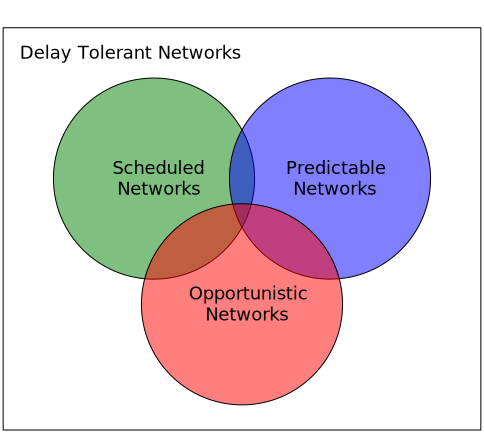
\includegraphics[width=0.5\textwidth]{Figures/TypeOfDTN.tikz}
\caption{Types of DTN}
\label{Type of DTN}
\end{figure} 
In the paper, the authors refer to the wildlife monitoring. 
%%
If it is one application that they suppose, they should consider the simulation model based on it. 
%%
The reviewer’s feeling is that the simulation model is too generic, and the readers could not have a confidence that the proposed method is useful. 
%%
The same argument can be applied to the predictable behavior of OppNet nodes. 
%%
Its applicability must be heavily dependent on the target system.
%%
Perhaps a more realistic realization is to use mobile robots to collect information around the field. 
%%
Even in the sparse environment, the path planning method can make the delivery ratio of packets higher. 
%%
See the related papers.

\begin{figure}[h]
\centering
\includegraphics[width=0.9\textwidth]{Figures/Spectrum.pdf}
\caption{A spectrum of contact schedule predictability}
\label{A spectrum of contact schedule predictability}
\end{figure} 

\problemAnswer{ % Answer

It is true that with the predictability capability of receiving nodes, the delivery ratio of packets can be increased.
%%
In the DTN (Delay Tolerant Network) researches, there are several proposals of using the concept of mobile robots such as Data MULES \cite{Jain2006,Tseng2013} where the MULES nodes move around a sensor network to gather sensing data or Message-Ferries \cite{Moazzez2013,Zhao2003,Zhao2004,Zhao2005} where the source passes the messages to a moving node that carries it directly to the destination or the DTMN (Delay Tolerant Mobile Network) \cite{Harras2005} with the self configured mobile nodes as a scheduled messenger moving along the design route. 

However, aforementioned controlled mobility algorithms are focus on the scheduled or predictable networks which are subtypes of DTN as in Fig. \ref{Type of DTN}.
%%
Our research is focused on the Opportunistic Networks where the movements of mobile nodes are completely random.
%%
Therefore, the path planning for a controllable mobile node is extremely difficult as can be seen in Fig. \ref{A spectrum of contact schedule predictability}.
%%
Nevertheless, we have shown the concept of path planning with our Predicable behavior OppNet nodes on the Rendezvous place searching algorithms where the movements of the nodes can be predicted and the routing of mobile robots can be planned.

In addition, our simulation model is based on the movements of animals where their movements are in the grouping behavior.
%%
We have used the Group movement model instead of common Random Way-point or Random Walk movement models which are the most widely use in the opportunistic routing simulations.
%%
The key idea of this paper is to address the randomness and spareness of the extreme environment by creating a Rendezvous or a meeting points where the nodes can efficiently exchange information carried with them without mainly depend on the predictability capability of controllable nodes.
}
\end{homeworkSection}
%------------------------------------------------------------------------------------

\begin{homeworkSection}{[Question 3]} % Section within problem
In summary, for the paper to be accepted, the authors clearly describe the application of the proposed method, and show the simulation results based on the application scenarios. Also, they should discuss why the proposed method is better than the other methods including the planning method using the mobile robots.

\problemAnswer{ % Answer
The applications of our proposed method can be deployed as wildlife monitoring or military operation scenario where the movement of the mobile nodes is in a group movement model.
%%
Our simulations are based on these scenarios where the operational area is sparse with two different approaches of searching algorithms: planing (Predictable behavior OppNet nodes) and without plan (Non-Predictable behavior OppNet nodes).
%%
The benefit of our proposed method comparing to other mobile robots is in the sense that our method does not mainly depend on the controlled mobility algorithms which can subject to the central point of failure (the network is down if the mobile robot cannot function properly).
%%
On the contrary, our proposed method aims to create a zone where the mobile nodes can deposit and pickup their messages without having to get contact with each other.
%%
Additionally, the planning method can be used with our proposed Rendezvous node if the scenario of mobile nodes can be predicted.

}
\end{homeworkSection}

\end{homeworkProblem}

\clearpage
%------------------------------------------------------------------------------------
%	Reviewer2
%------------------------------------------------------------------------------------


\begin{homeworkProblem}

This manuscript proposed a concept of rendezvous place for improving delivery ratio and reducing energy consumption in sparse opportunistic networks. 
%%
But some details are still unclear.
%----------------------------------------------------------------------------------------

\begin{homeworkSection}{[Question 1]} % Section within problem
How long could a message stay in the Rendezvous node buffer, if the Rendezvous node didn't encounter the target node? 

\problemAnswer{ % Answer
In the opportunistic network environments, a message is commonly embedded with a time-to-live (TTL) parameter (or called a message deadline) which stops the packets from traveling unnecessarily throughout the network \cite{Prodhan2011,Yuan2012,Nguyen2009,Khabbaz2012}. 
%
Our provious work \cite{Kerdsri2013} has shown that the different value of message deadlines can affect the delivery ratio. 
%
In our design, each message will be dropped once it reach the message deadline in order to clear the messages left on the buffer of Rendezvous node.
%%
If the capacity of data storage in Rendezvous node is fully occupied, then the oldest messages will be dropped once the new messages arrives.
%%
In our simulation, we setup the TTL to the simulation time in order to hold the messages in the Rendezvous zone as long as possible.
%%
We assume that Rendezvous buffer is large enough to feasible store as many messages waiting to pickup by target nodes.
%%
Therefore, the messages will indefinitely stay in the Rendezvous node buffer until the storage is full and the newer messages request the space from the buffer.
}
\end{homeworkSection}
%------------------------------------------------------------------------------------

\begin{homeworkSection}{[Question 2]} % Section within problem
If the Rendezvous node can't find the expected node-gathering area for a long time, does it keep moving? In this process, is it broadcasting the Rendezvous Area rumor message (RA)? 

\problemAnswer{ % Answer
In our system, the Rendezvous node will move to a new location if there is insufficient contact from OppNet node within a predefined duration.
%
Consequently,the Rendezvous node will situate in the node-gathering area when there is enough number of encountered OppNet nodes.
%%
Therefore, the Rendezvous nodes will keep moving until they meet the desired conditions.
%%
In addition, in the process of moving, the Rendezvous node will keep broadcasting the Rendezvous Area rumor message ($RA$), so the OppNet nodes can learn that they are in the Rendezvous zone when they detect the $RA$ messages. 
}
\end{homeworkSection}
%------------------------------------------------------------------------------------

\begin{homeworkSection}{[Question 3]} % Section within problem
Moreover, how does it determine its center location when implementing sweeping algorithm? How do you see the relationship between the period of sweep mechanism and the period of searching Rendezvous place?

\begin{figure}[h]
\centering
\includegraphics[width=1.5in]{Figures/Sweep.pdf}
\caption{Sweep mechanism}
\label{Sweep mechanism}
\end{figure}

\problemAnswer{ % Answer
The sweeping mechanism is started when the Rendezvous node station in the desire location in order to gain more delivery ratio from the nodes with different transmission range.
%%
The center location of Rendezvous for the sweeping algorithm is determined by its radio range since the Rendezvous node can move to 4 direction as in Fig. \ref{Sweep mechanism}.
%%
The period of sweep mechanism and searching Rendezvous place are irrelevant since the sweeping always performs when the Rendezvous node is stationed while the period of searching is depended on the encountered OppNet nodes.
}
\end{homeworkSection}
%------------------------------------------------------------------------------------

\begin{homeworkSection}{[Question 4]} % Section within problem
The Rendezvous node should passively wait for the target node entering the Rendezvous place. Does it harm the efficiency of packet delivery, compared with some latest opportunistic routings?

\problemAnswer{ % Answer
In our implementation, the Rendezvous node can move with the Sweep mechanism to gain more chance of meeting the node with less transmission radio range.
%%
Thus, this mechanism can increase the performance of packet delivery while most of the recent opportunistic routings such as Throwbox \cite{Zhu2014,Banerjee2010} or passive relay points \cite{Shahbazi2012} which recieving base station are more passively waiting for the contact nodes. 
}
\end{homeworkSection}
%------------------------------------------------------------------------------------
\begin{figure}[h]
	\centering
% Graphic for TeX using PGF
% Title: /Users/Arm/Desktop/Diagram1.dia
% Creator: Dia v0.97.2
% CreationDate: Fri Sep 12 16:02:14 2014
% For: Arm
% \usepackage{tikz}
% The following commands are not supported in PSTricks at present
% We define them conditionally, so when they are implemented,
% this pgf file will use them.
\ifx\du\undefined
  \newlength{\du}
\fi
\setlength{\du}{15\unitlength}
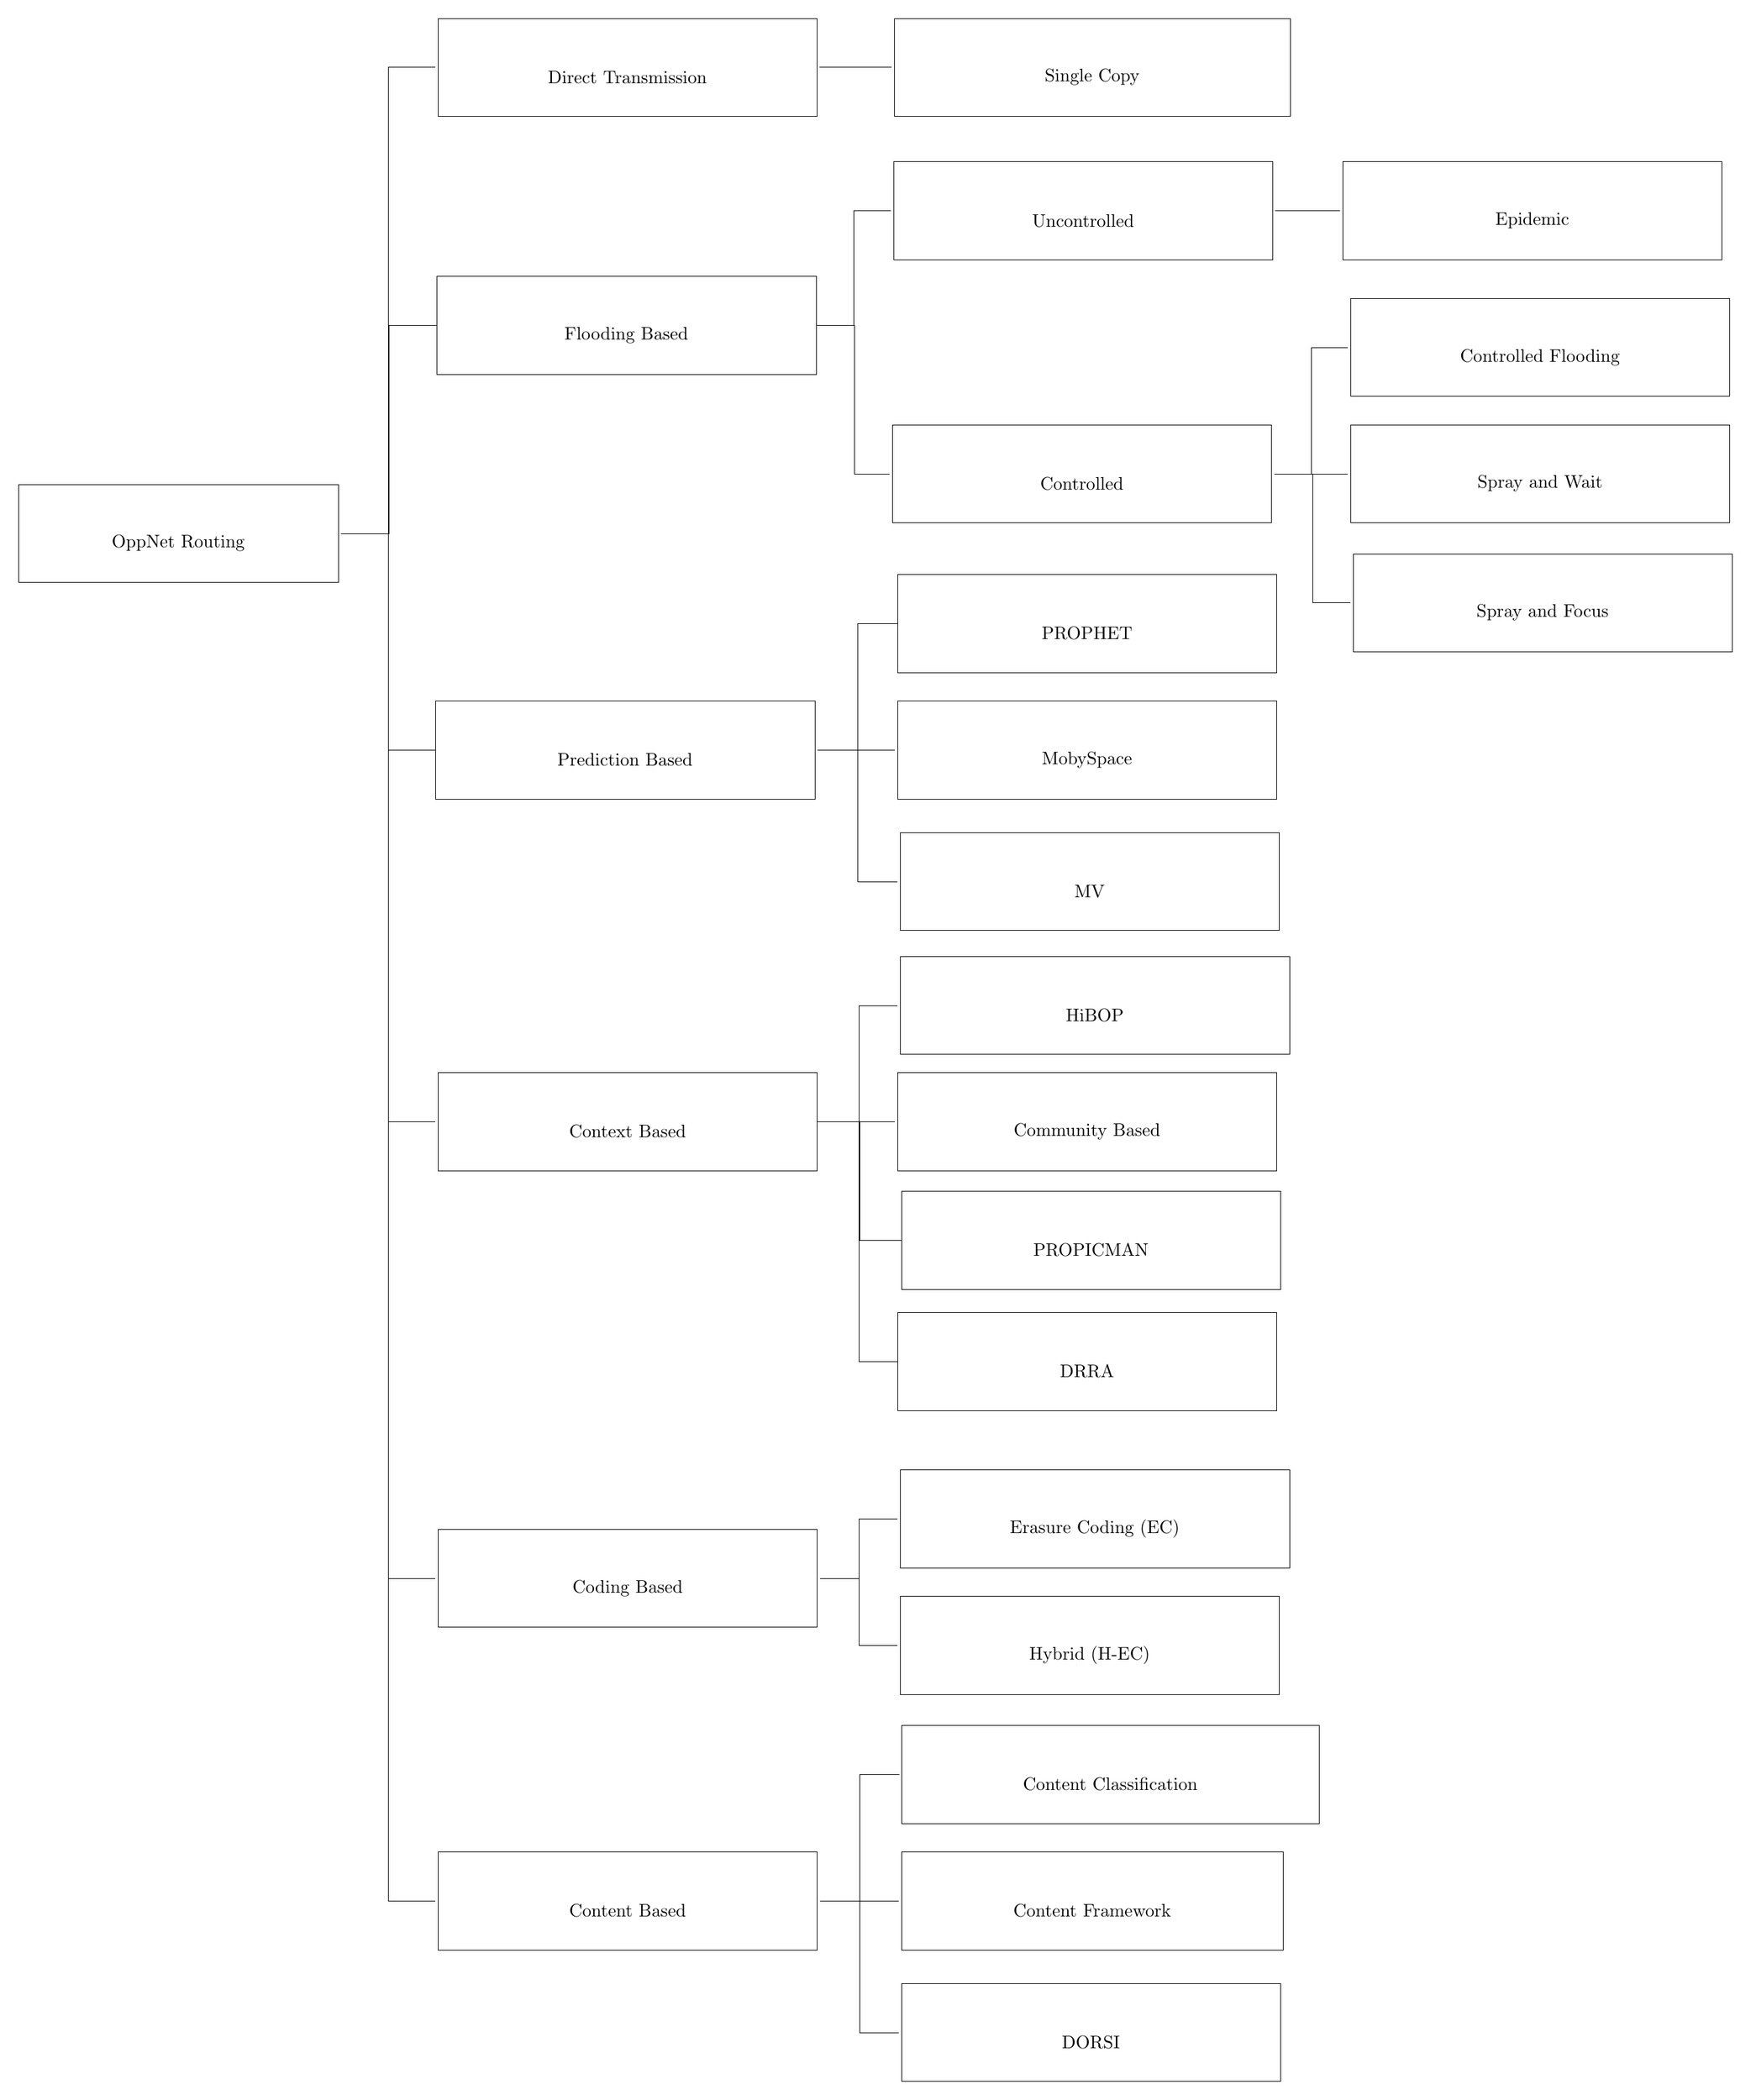
\begin{tikzpicture}
\pgftransformxscale{1.000000}
\pgftransformyscale{-1.000000}
\definecolor{dialinecolor}{rgb}{0.000000, 0.000000, 0.000000}
\pgfsetstrokecolor{dialinecolor}
\definecolor{dialinecolor}{rgb}{1.000000, 1.000000, 1.000000}
\pgfsetfillcolor{dialinecolor}
\definecolor{dialinecolor}{rgb}{1.000000, 1.000000, 1.000000}
\pgfsetfillcolor{dialinecolor}
\fill (3.606250\du,23.050000\du)--(3.606250\du,24.950000\du)--(9.808750\du,24.950000\du)--(9.808750\du,23.050000\du)--cycle;
\pgfsetlinewidth{0.100000\du}
\pgfsetdash{}{0pt}
\pgfsetdash{}{0pt}
\pgfsetmiterjoin
\definecolor{dialinecolor}{rgb}{0.000000, 0.000000, 0.000000}
\pgfsetstrokecolor{dialinecolor}
\draw (3.606250\du,23.050000\du)--(3.606250\du,24.950000\du)--(9.808750\du,24.950000\du)--(9.808750\du,23.050000\du)--cycle;
% setfont left to latex
\definecolor{dialinecolor}{rgb}{0.000000, 0.000000, 0.000000}
\pgfsetstrokecolor{dialinecolor}
\node at (6.707500\du,24.195000\du){OppNet Routing};
\definecolor{dialinecolor}{rgb}{1.000000, 1.000000, 1.000000}
\pgfsetfillcolor{dialinecolor}
\fill (11.736200\du,14.020000\du)--(11.736200\du,15.920000\du)--(19.081200\du,15.920000\du)--(19.081200\du,14.020000\du)--cycle;
\pgfsetlinewidth{0.100000\du}
\pgfsetdash{}{0pt}
\pgfsetdash{}{0pt}
\pgfsetmiterjoin
\definecolor{dialinecolor}{rgb}{0.000000, 0.000000, 0.000000}
\pgfsetstrokecolor{dialinecolor}
\draw (11.736200\du,14.020000\du)--(11.736200\du,15.920000\du)--(19.081200\du,15.920000\du)--(19.081200\du,14.020000\du)--cycle;
% setfont left to latex
\definecolor{dialinecolor}{rgb}{0.000000, 0.000000, 0.000000}
\pgfsetstrokecolor{dialinecolor}
\node at (15.408700\du,15.165000\du){Direct Transmission};
\pgfsetlinewidth{0.100000\du}
\pgfsetdash{}{0pt}
\pgfsetdash{}{0pt}
\pgfsetmiterjoin
\pgfsetbuttcap
{
\definecolor{dialinecolor}{rgb}{0.000000, 0.000000, 0.000000}
\pgfsetfillcolor{dialinecolor}
% was here!!!
{\pgfsetcornersarced{\pgfpoint{0.000000\du}{0.000000\du}}\definecolor{dialinecolor}{rgb}{0.000000, 0.000000, 0.000000}
\pgfsetstrokecolor{dialinecolor}
\draw (9.859135\du,24.000000\du)--(10.772440\du,24.000000\du)--(10.772440\du,14.970000\du)--(11.685746\du,14.970000\du);
}}
\definecolor{dialinecolor}{rgb}{1.000000, 1.000000, 1.000000}
\pgfsetfillcolor{dialinecolor}
\fill (20.574100\du,14.020000\du)--(20.574100\du,15.920000\du)--(28.250804\du,15.920000\du)--(28.250804\du,14.020000\du)--cycle;
\pgfsetlinewidth{0.100000\du}
\pgfsetdash{}{0pt}
\pgfsetdash{}{0pt}
\pgfsetmiterjoin
\definecolor{dialinecolor}{rgb}{0.000000, 0.000000, 0.000000}
\pgfsetstrokecolor{dialinecolor}
\draw (20.574100\du,14.020000\du)--(20.574100\du,15.920000\du)--(28.250804\du,15.920000\du)--(28.250804\du,14.020000\du)--cycle;
% setfont left to latex
\definecolor{dialinecolor}{rgb}{0.000000, 0.000000, 0.000000}
\pgfsetstrokecolor{dialinecolor}
\node at (24.412452\du,15.165000\du){Single Copy};
\pgfsetlinewidth{0.100000\du}
\pgfsetdash{}{0pt}
\pgfsetdash{}{0pt}
\pgfsetmiterjoin
\pgfsetbuttcap
{
\definecolor{dialinecolor}{rgb}{0.000000, 0.000000, 0.000000}
\pgfsetfillcolor{dialinecolor}
% was here!!!
{\pgfsetcornersarced{\pgfpoint{0.000000\du}{0.000000\du}}\definecolor{dialinecolor}{rgb}{0.000000, 0.000000, 0.000000}
\pgfsetstrokecolor{dialinecolor}
\draw (19.131654\du,14.970000\du)--(19.181654\du,14.970000\du)--(20.473625\du,14.970000\du)--(20.523625\du,14.970000\du);
}}
\definecolor{dialinecolor}{rgb}{1.000000, 1.000000, 1.000000}
\pgfsetfillcolor{dialinecolor}
\fill (11.715000\du,19.020000\du)--(11.715000\du,20.920000\du)--(19.060000\du,20.920000\du)--(19.060000\du,19.020000\du)--cycle;
\pgfsetlinewidth{0.100000\du}
\pgfsetdash{}{0pt}
\pgfsetdash{}{0pt}
\pgfsetmiterjoin
\definecolor{dialinecolor}{rgb}{0.000000, 0.000000, 0.000000}
\pgfsetstrokecolor{dialinecolor}
\draw (11.715000\du,19.020000\du)--(11.715000\du,20.920000\du)--(19.060000\du,20.920000\du)--(19.060000\du,19.020000\du)--cycle;
% setfont left to latex
\definecolor{dialinecolor}{rgb}{0.000000, 0.000000, 0.000000}
\pgfsetstrokecolor{dialinecolor}
\node at (15.387500\du,20.165000\du){Flooding Based};
\definecolor{dialinecolor}{rgb}{1.000000, 1.000000, 1.000000}
\pgfsetfillcolor{dialinecolor}
\fill (20.565000\du,16.795000\du)--(20.565000\du,18.695000\du)--(27.910000\du,18.695000\du)--(27.910000\du,16.795000\du)--cycle;
\pgfsetlinewidth{0.100000\du}
\pgfsetdash{}{0pt}
\pgfsetdash{}{0pt}
\pgfsetmiterjoin
\definecolor{dialinecolor}{rgb}{0.000000, 0.000000, 0.000000}
\pgfsetstrokecolor{dialinecolor}
\draw (20.565000\du,16.795000\du)--(20.565000\du,18.695000\du)--(27.910000\du,18.695000\du)--(27.910000\du,16.795000\du)--cycle;
% setfont left to latex
\definecolor{dialinecolor}{rgb}{0.000000, 0.000000, 0.000000}
\pgfsetstrokecolor{dialinecolor}
\node at (24.237500\du,17.940000\du){Uncontrolled};
\definecolor{dialinecolor}{rgb}{1.000000, 1.000000, 1.000000}
\pgfsetfillcolor{dialinecolor}
\fill (20.540000\du,21.895000\du)--(20.540000\du,23.795000\du)--(27.885000\du,23.795000\du)--(27.885000\du,21.895000\du)--cycle;
\pgfsetlinewidth{0.100000\du}
\pgfsetdash{}{0pt}
\pgfsetdash{}{0pt}
\pgfsetmiterjoin
\definecolor{dialinecolor}{rgb}{0.000000, 0.000000, 0.000000}
\pgfsetstrokecolor{dialinecolor}
\draw (20.540000\du,21.895000\du)--(20.540000\du,23.795000\du)--(27.885000\du,23.795000\du)--(27.885000\du,21.895000\du)--cycle;
% setfont left to latex
\definecolor{dialinecolor}{rgb}{0.000000, 0.000000, 0.000000}
\pgfsetstrokecolor{dialinecolor}
\node at (24.212500\du,23.040000\du){Controlled};
\definecolor{dialinecolor}{rgb}{1.000000, 1.000000, 1.000000}
\pgfsetfillcolor{dialinecolor}
\fill (29.265000\du,16.795000\du)--(29.265000\du,18.695000\du)--(36.610000\du,18.695000\du)--(36.610000\du,16.795000\du)--cycle;
\pgfsetlinewidth{0.100000\du}
\pgfsetdash{}{0pt}
\pgfsetdash{}{0pt}
\pgfsetmiterjoin
\definecolor{dialinecolor}{rgb}{0.000000, 0.000000, 0.000000}
\pgfsetstrokecolor{dialinecolor}
\draw (29.265000\du,16.795000\du)--(29.265000\du,18.695000\du)--(36.610000\du,18.695000\du)--(36.610000\du,16.795000\du)--cycle;
% setfont left to latex
\definecolor{dialinecolor}{rgb}{0.000000, 0.000000, 0.000000}
\pgfsetstrokecolor{dialinecolor}
\node at (32.937500\du,17.940000\du){Epidemic};
\pgfsetlinewidth{0.100000\du}
\pgfsetdash{}{0pt}
\pgfsetdash{}{0pt}
\pgfsetmiterjoin
\pgfsetbuttcap
{
\definecolor{dialinecolor}{rgb}{0.000000, 0.000000, 0.000000}
\pgfsetfillcolor{dialinecolor}
% was here!!!
{\pgfsetcornersarced{\pgfpoint{0.000000\du}{0.000000\du}}\definecolor{dialinecolor}{rgb}{0.000000, 0.000000, 0.000000}
\pgfsetstrokecolor{dialinecolor}
\draw (9.859135\du,24.000000\du)--(10.787067\du,24.000000\du)--(10.787067\du,19.970000\du)--(11.715000\du,19.970000\du);
}}
\pgfsetlinewidth{0.100000\du}
\pgfsetdash{}{0pt}
\pgfsetdash{}{0pt}
\pgfsetmiterjoin
\pgfsetbuttcap
{
\definecolor{dialinecolor}{rgb}{0.000000, 0.000000, 0.000000}
\pgfsetfillcolor{dialinecolor}
% was here!!!
{\pgfsetcornersarced{\pgfpoint{0.000000\du}{0.000000\du}}\definecolor{dialinecolor}{rgb}{0.000000, 0.000000, 0.000000}
\pgfsetstrokecolor{dialinecolor}
\draw (19.060000\du,19.970000\du)--(19.787273\du,19.970000\du)--(19.787273\du,17.745000\du)--(20.514546\du,17.745000\du);
}}
\pgfsetlinewidth{0.100000\du}
\pgfsetdash{}{0pt}
\pgfsetdash{}{0pt}
\pgfsetmiterjoin
\pgfsetbuttcap
{
\definecolor{dialinecolor}{rgb}{0.000000, 0.000000, 0.000000}
\pgfsetfillcolor{dialinecolor}
% was here!!!
{\pgfsetcornersarced{\pgfpoint{0.000000\du}{0.000000\du}}\definecolor{dialinecolor}{rgb}{0.000000, 0.000000, 0.000000}
\pgfsetstrokecolor{dialinecolor}
\draw (19.110454\du,19.970000\du)--(19.800000\du,19.970000\du)--(19.800000\du,22.845000\du)--(20.489546\du,22.845000\du);
}}
\pgfsetlinewidth{0.100000\du}
\pgfsetdash{}{0pt}
\pgfsetdash{}{0pt}
\pgfsetmiterjoin
\pgfsetbuttcap
{
\definecolor{dialinecolor}{rgb}{0.000000, 0.000000, 0.000000}
\pgfsetfillcolor{dialinecolor}
% was here!!!
{\pgfsetcornersarced{\pgfpoint{0.000000\du}{0.000000\du}}\definecolor{dialinecolor}{rgb}{0.000000, 0.000000, 0.000000}
\pgfsetstrokecolor{dialinecolor}
\draw (27.960454\du,17.745000\du)--(28.010454\du,17.745000\du)--(29.164546\du,17.745000\du)--(29.214546\du,17.745000\du);
}}
\definecolor{dialinecolor}{rgb}{1.000000, 1.000000, 1.000000}
\pgfsetfillcolor{dialinecolor}
\fill (29.415000\du,19.445000\du)--(29.415000\du,21.345000\du)--(36.760000\du,21.345000\du)--(36.760000\du,19.445000\du)--cycle;
\pgfsetlinewidth{0.100000\du}
\pgfsetdash{}{0pt}
\pgfsetdash{}{0pt}
\pgfsetmiterjoin
\definecolor{dialinecolor}{rgb}{0.000000, 0.000000, 0.000000}
\pgfsetstrokecolor{dialinecolor}
\draw (29.415000\du,19.445000\du)--(29.415000\du,21.345000\du)--(36.760000\du,21.345000\du)--(36.760000\du,19.445000\du)--cycle;
% setfont left to latex
\definecolor{dialinecolor}{rgb}{0.000000, 0.000000, 0.000000}
\pgfsetstrokecolor{dialinecolor}
\node at (33.087500\du,20.590000\du){Controlled Flooding};
\definecolor{dialinecolor}{rgb}{1.000000, 1.000000, 1.000000}
\pgfsetfillcolor{dialinecolor}
\fill (29.415000\du,21.895000\du)--(29.415000\du,23.795000\du)--(36.760000\du,23.795000\du)--(36.760000\du,21.895000\du)--cycle;
\pgfsetlinewidth{0.100000\du}
\pgfsetdash{}{0pt}
\pgfsetdash{}{0pt}
\pgfsetmiterjoin
\definecolor{dialinecolor}{rgb}{0.000000, 0.000000, 0.000000}
\pgfsetstrokecolor{dialinecolor}
\draw (29.415000\du,21.895000\du)--(29.415000\du,23.795000\du)--(36.760000\du,23.795000\du)--(36.760000\du,21.895000\du)--cycle;
% setfont left to latex
\definecolor{dialinecolor}{rgb}{0.000000, 0.000000, 0.000000}
\pgfsetstrokecolor{dialinecolor}
\node at (33.087500\du,23.040000\du){Spray and Wait};
\definecolor{dialinecolor}{rgb}{1.000000, 1.000000, 1.000000}
\pgfsetfillcolor{dialinecolor}
\fill (29.465000\du,24.395000\du)--(29.465000\du,26.295000\du)--(36.810000\du,26.295000\du)--(36.810000\du,24.395000\du)--cycle;
\pgfsetlinewidth{0.100000\du}
\pgfsetdash{}{0pt}
\pgfsetdash{}{0pt}
\pgfsetmiterjoin
\definecolor{dialinecolor}{rgb}{0.000000, 0.000000, 0.000000}
\pgfsetstrokecolor{dialinecolor}
\draw (29.465000\du,24.395000\du)--(29.465000\du,26.295000\du)--(36.810000\du,26.295000\du)--(36.810000\du,24.395000\du)--cycle;
% setfont left to latex
\definecolor{dialinecolor}{rgb}{0.000000, 0.000000, 0.000000}
\pgfsetstrokecolor{dialinecolor}
\node at (33.137500\du,25.540000\du){Spray and Focus};
\pgfsetlinewidth{0.100000\du}
\pgfsetdash{}{0pt}
\pgfsetdash{}{0pt}
\pgfsetmiterjoin
\pgfsetbuttcap
{
\definecolor{dialinecolor}{rgb}{0.000000, 0.000000, 0.000000}
\pgfsetfillcolor{dialinecolor}
% was here!!!
{\pgfsetcornersarced{\pgfpoint{0.000000\du}{0.000000\du}}\definecolor{dialinecolor}{rgb}{0.000000, 0.000000, 0.000000}
\pgfsetstrokecolor{dialinecolor}
\draw (27.935454\du,22.845000\du)--(28.650000\du,22.845000\du)--(28.650000\du,20.395000\du)--(29.364546\du,20.395000\du);
}}
\pgfsetlinewidth{0.100000\du}
\pgfsetdash{}{0pt}
\pgfsetdash{}{0pt}
\pgfsetmiterjoin
\pgfsetbuttcap
{
\definecolor{dialinecolor}{rgb}{0.000000, 0.000000, 0.000000}
\pgfsetfillcolor{dialinecolor}
% was here!!!
{\pgfsetcornersarced{\pgfpoint{0.000000\du}{0.000000\du}}\definecolor{dialinecolor}{rgb}{0.000000, 0.000000, 0.000000}
\pgfsetstrokecolor{dialinecolor}
\draw (27.935454\du,22.845000\du)--(27.985454\du,22.845000\du)--(29.314546\du,22.845000\du)--(29.364546\du,22.845000\du);
}}
\pgfsetlinewidth{0.100000\du}
\pgfsetdash{}{0pt}
\pgfsetdash{}{0pt}
\pgfsetmiterjoin
\pgfsetbuttcap
{
\definecolor{dialinecolor}{rgb}{0.000000, 0.000000, 0.000000}
\pgfsetfillcolor{dialinecolor}
% was here!!!
{\pgfsetcornersarced{\pgfpoint{0.000000\du}{0.000000\du}}\definecolor{dialinecolor}{rgb}{0.000000, 0.000000, 0.000000}
\pgfsetstrokecolor{dialinecolor}
\draw (27.935454\du,22.845000\du)--(28.675000\du,22.845000\du)--(28.675000\du,25.345000\du)--(29.414546\du,25.345000\du);
}}
\definecolor{dialinecolor}{rgb}{1.000000, 1.000000, 1.000000}
\pgfsetfillcolor{dialinecolor}
\fill (11.690000\du,27.245000\du)--(11.690000\du,29.145000\du)--(19.035000\du,29.145000\du)--(19.035000\du,27.245000\du)--cycle;
\pgfsetlinewidth{0.100000\du}
\pgfsetdash{}{0pt}
\pgfsetdash{}{0pt}
\pgfsetmiterjoin
\definecolor{dialinecolor}{rgb}{0.000000, 0.000000, 0.000000}
\pgfsetstrokecolor{dialinecolor}
\draw (11.690000\du,27.245000\du)--(11.690000\du,29.145000\du)--(19.035000\du,29.145000\du)--(19.035000\du,27.245000\du)--cycle;
% setfont left to latex
\definecolor{dialinecolor}{rgb}{0.000000, 0.000000, 0.000000}
\pgfsetstrokecolor{dialinecolor}
\node at (15.362500\du,28.390000\du){Prediction Based};
\definecolor{dialinecolor}{rgb}{1.000000, 1.000000, 1.000000}
\pgfsetfillcolor{dialinecolor}
\fill (20.640000\du,24.795000\du)--(20.640000\du,26.695000\du)--(27.985000\du,26.695000\du)--(27.985000\du,24.795000\du)--cycle;
\pgfsetlinewidth{0.100000\du}
\pgfsetdash{}{0pt}
\pgfsetdash{}{0pt}
\pgfsetmiterjoin
\definecolor{dialinecolor}{rgb}{0.000000, 0.000000, 0.000000}
\pgfsetstrokecolor{dialinecolor}
\draw (20.640000\du,24.795000\du)--(20.640000\du,26.695000\du)--(27.985000\du,26.695000\du)--(27.985000\du,24.795000\du)--cycle;
% setfont left to latex
\definecolor{dialinecolor}{rgb}{0.000000, 0.000000, 0.000000}
\pgfsetstrokecolor{dialinecolor}
\node at (24.312500\du,25.940000\du){PROPHET};
\definecolor{dialinecolor}{rgb}{1.000000, 1.000000, 1.000000}
\pgfsetfillcolor{dialinecolor}
\fill (20.640000\du,27.245000\du)--(20.640000\du,29.145000\du)--(27.985000\du,29.145000\du)--(27.985000\du,27.245000\du)--cycle;
\pgfsetlinewidth{0.100000\du}
\pgfsetdash{}{0pt}
\pgfsetdash{}{0pt}
\pgfsetmiterjoin
\definecolor{dialinecolor}{rgb}{0.000000, 0.000000, 0.000000}
\pgfsetstrokecolor{dialinecolor}
\draw (20.640000\du,27.245000\du)--(20.640000\du,29.145000\du)--(27.985000\du,29.145000\du)--(27.985000\du,27.245000\du)--cycle;
% setfont left to latex
\definecolor{dialinecolor}{rgb}{0.000000, 0.000000, 0.000000}
\pgfsetstrokecolor{dialinecolor}
\node at (24.312500\du,28.390000\du){MobySpace};
\definecolor{dialinecolor}{rgb}{1.000000, 1.000000, 1.000000}
\pgfsetfillcolor{dialinecolor}
\fill (20.690000\du,29.795000\du)--(20.690000\du,31.695000\du)--(28.035000\du,31.695000\du)--(28.035000\du,29.795000\du)--cycle;
\pgfsetlinewidth{0.100000\du}
\pgfsetdash{}{0pt}
\pgfsetdash{}{0pt}
\pgfsetmiterjoin
\definecolor{dialinecolor}{rgb}{0.000000, 0.000000, 0.000000}
\pgfsetstrokecolor{dialinecolor}
\draw (20.690000\du,29.795000\du)--(20.690000\du,31.695000\du)--(28.035000\du,31.695000\du)--(28.035000\du,29.795000\du)--cycle;
% setfont left to latex
\definecolor{dialinecolor}{rgb}{0.000000, 0.000000, 0.000000}
\pgfsetstrokecolor{dialinecolor}
\node at (24.362500\du,30.940000\du){MV};
\pgfsetlinewidth{0.100000\du}
\pgfsetdash{}{0pt}
\pgfsetdash{}{0pt}
\pgfsetmiterjoin
\pgfsetbuttcap
{
\definecolor{dialinecolor}{rgb}{0.000000, 0.000000, 0.000000}
\pgfsetfillcolor{dialinecolor}
% was here!!!
{\pgfsetcornersarced{\pgfpoint{0.000000\du}{0.000000\du}}\definecolor{dialinecolor}{rgb}{0.000000, 0.000000, 0.000000}
\pgfsetstrokecolor{dialinecolor}
\draw (9.859135\du,24.000000\du)--(10.774567\du,24.000000\du)--(10.774567\du,28.195000\du)--(11.690000\du,28.195000\du);
}}
\pgfsetlinewidth{0.100000\du}
\pgfsetdash{}{0pt}
\pgfsetdash{}{0pt}
\pgfsetmiterjoin
\pgfsetbuttcap
{
\definecolor{dialinecolor}{rgb}{0.000000, 0.000000, 0.000000}
\pgfsetfillcolor{dialinecolor}
% was here!!!
{\pgfsetcornersarced{\pgfpoint{0.000000\du}{0.000000\du}}\definecolor{dialinecolor}{rgb}{0.000000, 0.000000, 0.000000}
\pgfsetstrokecolor{dialinecolor}
\draw (19.085454\du,28.195000\du)--(19.862727\du,28.195000\du)--(19.862727\du,25.745000\du)--(20.640000\du,25.745000\du);
}}
\pgfsetlinewidth{0.100000\du}
\pgfsetdash{}{0pt}
\pgfsetdash{}{0pt}
\pgfsetmiterjoin
\pgfsetbuttcap
{
\definecolor{dialinecolor}{rgb}{0.000000, 0.000000, 0.000000}
\pgfsetfillcolor{dialinecolor}
% was here!!!
{\pgfsetcornersarced{\pgfpoint{0.000000\du}{0.000000\du}}\definecolor{dialinecolor}{rgb}{0.000000, 0.000000, 0.000000}
\pgfsetstrokecolor{dialinecolor}
\draw (19.085454\du,28.195000\du)--(19.135454\du,28.195000\du)--(20.539546\du,28.195000\du)--(20.589546\du,28.195000\du);
}}
\pgfsetlinewidth{0.100000\du}
\pgfsetdash{}{0pt}
\pgfsetdash{}{0pt}
\pgfsetmiterjoin
\pgfsetbuttcap
{
\definecolor{dialinecolor}{rgb}{0.000000, 0.000000, 0.000000}
\pgfsetfillcolor{dialinecolor}
% was here!!!
{\pgfsetcornersarced{\pgfpoint{0.000000\du}{0.000000\du}}\definecolor{dialinecolor}{rgb}{0.000000, 0.000000, 0.000000}
\pgfsetstrokecolor{dialinecolor}
\draw (19.085454\du,28.195000\du)--(19.862500\du,28.195000\du)--(19.862500\du,30.745000\du)--(20.639546\du,30.745000\du);
}}
\definecolor{dialinecolor}{rgb}{1.000000, 1.000000, 1.000000}
\pgfsetfillcolor{dialinecolor}
\fill (11.740000\du,43.295000\du)--(11.740000\du,45.195000\du)--(19.085000\du,45.195000\du)--(19.085000\du,43.295000\du)--cycle;
\pgfsetlinewidth{0.100000\du}
\pgfsetdash{}{0pt}
\pgfsetdash{}{0pt}
\pgfsetmiterjoin
\definecolor{dialinecolor}{rgb}{0.000000, 0.000000, 0.000000}
\pgfsetstrokecolor{dialinecolor}
\draw (11.740000\du,43.295000\du)--(11.740000\du,45.195000\du)--(19.085000\du,45.195000\du)--(19.085000\du,43.295000\du)--cycle;
% setfont left to latex
\definecolor{dialinecolor}{rgb}{0.000000, 0.000000, 0.000000}
\pgfsetstrokecolor{dialinecolor}
\node at (15.412500\du,44.440000\du){Coding Based};
\definecolor{dialinecolor}{rgb}{1.000000, 1.000000, 1.000000}
\pgfsetfillcolor{dialinecolor}
\fill (20.695000\du,42.145000\du)--(20.695000\du,44.045000\du)--(28.230000\du,44.045000\du)--(28.230000\du,42.145000\du)--cycle;
\pgfsetlinewidth{0.100000\du}
\pgfsetdash{}{0pt}
\pgfsetdash{}{0pt}
\pgfsetmiterjoin
\definecolor{dialinecolor}{rgb}{0.000000, 0.000000, 0.000000}
\pgfsetstrokecolor{dialinecolor}
\draw (20.695000\du,42.145000\du)--(20.695000\du,44.045000\du)--(28.230000\du,44.045000\du)--(28.230000\du,42.145000\du)--cycle;
% setfont left to latex
\definecolor{dialinecolor}{rgb}{0.000000, 0.000000, 0.000000}
\pgfsetstrokecolor{dialinecolor}
\node at (24.462500\du,43.290000\du){Erasure Coding (EC)};
\definecolor{dialinecolor}{rgb}{1.000000, 1.000000, 1.000000}
\pgfsetfillcolor{dialinecolor}
\fill (20.690000\du,44.595000\du)--(20.690000\du,46.495000\du)--(28.035000\du,46.495000\du)--(28.035000\du,44.595000\du)--cycle;
\pgfsetlinewidth{0.100000\du}
\pgfsetdash{}{0pt}
\pgfsetdash{}{0pt}
\pgfsetmiterjoin
\definecolor{dialinecolor}{rgb}{0.000000, 0.000000, 0.000000}
\pgfsetstrokecolor{dialinecolor}
\draw (20.690000\du,44.595000\du)--(20.690000\du,46.495000\du)--(28.035000\du,46.495000\du)--(28.035000\du,44.595000\du)--cycle;
% setfont left to latex
\definecolor{dialinecolor}{rgb}{0.000000, 0.000000, 0.000000}
\pgfsetstrokecolor{dialinecolor}
\node at (24.362500\du,45.740000\du){Hybrid (H-EC)};
\pgfsetlinewidth{0.100000\du}
\pgfsetdash{}{0pt}
\pgfsetdash{}{0pt}
\pgfsetmiterjoin
\pgfsetbuttcap
{
\definecolor{dialinecolor}{rgb}{0.000000, 0.000000, 0.000000}
\pgfsetfillcolor{dialinecolor}
% was here!!!
{\pgfsetcornersarced{\pgfpoint{0.000000\du}{0.000000\du}}\definecolor{dialinecolor}{rgb}{0.000000, 0.000000, 0.000000}
\pgfsetstrokecolor{dialinecolor}
\draw (9.859135\du,24.000000\du)--(10.774340\du,24.000000\du)--(10.774340\du,44.245000\du)--(11.689546\du,44.245000\du);
}}
\pgfsetlinewidth{0.100000\du}
\pgfsetdash{}{0pt}
\pgfsetdash{}{0pt}
\pgfsetmiterjoin
\pgfsetbuttcap
{
\definecolor{dialinecolor}{rgb}{0.000000, 0.000000, 0.000000}
\pgfsetfillcolor{dialinecolor}
% was here!!!
{\pgfsetcornersarced{\pgfpoint{0.000000\du}{0.000000\du}}\definecolor{dialinecolor}{rgb}{0.000000, 0.000000, 0.000000}
\pgfsetstrokecolor{dialinecolor}
\draw (19.135454\du,44.245000\du)--(19.889994\du,44.245000\du)--(19.889994\du,43.095000\du)--(20.644534\du,43.095000\du);
}}
\pgfsetlinewidth{0.100000\du}
\pgfsetdash{}{0pt}
\pgfsetdash{}{0pt}
\pgfsetmiterjoin
\pgfsetbuttcap
{
\definecolor{dialinecolor}{rgb}{0.000000, 0.000000, 0.000000}
\pgfsetfillcolor{dialinecolor}
% was here!!!
{\pgfsetcornersarced{\pgfpoint{0.000000\du}{0.000000\du}}\definecolor{dialinecolor}{rgb}{0.000000, 0.000000, 0.000000}
\pgfsetstrokecolor{dialinecolor}
\draw (19.135454\du,44.245000\du)--(19.887500\du,44.245000\du)--(19.887500\du,45.545000\du)--(20.639546\du,45.545000\du);
}}
\definecolor{dialinecolor}{rgb}{1.000000, 1.000000, 1.000000}
\pgfsetfillcolor{dialinecolor}
\fill (11.740000\du,34.445000\du)--(11.740000\du,36.345000\du)--(19.085000\du,36.345000\du)--(19.085000\du,34.445000\du)--cycle;
\pgfsetlinewidth{0.100000\du}
\pgfsetdash{}{0pt}
\pgfsetdash{}{0pt}
\pgfsetmiterjoin
\definecolor{dialinecolor}{rgb}{0.000000, 0.000000, 0.000000}
\pgfsetstrokecolor{dialinecolor}
\draw (11.740000\du,34.445000\du)--(11.740000\du,36.345000\du)--(19.085000\du,36.345000\du)--(19.085000\du,34.445000\du)--cycle;
% setfont left to latex
\definecolor{dialinecolor}{rgb}{0.000000, 0.000000, 0.000000}
\pgfsetstrokecolor{dialinecolor}
\node at (15.412500\du,35.590000\du){Context Based};
\definecolor{dialinecolor}{rgb}{1.000000, 1.000000, 1.000000}
\pgfsetfillcolor{dialinecolor}
\fill (20.695000\du,32.195000\du)--(20.695000\du,34.095000\du)--(28.230000\du,34.095000\du)--(28.230000\du,32.195000\du)--cycle;
\pgfsetlinewidth{0.100000\du}
\pgfsetdash{}{0pt}
\pgfsetdash{}{0pt}
\pgfsetmiterjoin
\definecolor{dialinecolor}{rgb}{0.000000, 0.000000, 0.000000}
\pgfsetstrokecolor{dialinecolor}
\draw (20.695000\du,32.195000\du)--(20.695000\du,34.095000\du)--(28.230000\du,34.095000\du)--(28.230000\du,32.195000\du)--cycle;
% setfont left to latex
\definecolor{dialinecolor}{rgb}{0.000000, 0.000000, 0.000000}
\pgfsetstrokecolor{dialinecolor}
\node at (24.462500\du,33.340000\du){HiBOP};
\definecolor{dialinecolor}{rgb}{1.000000, 1.000000, 1.000000}
\pgfsetfillcolor{dialinecolor}
\fill (20.640000\du,34.445000\du)--(20.640000\du,36.345000\du)--(27.985000\du,36.345000\du)--(27.985000\du,34.445000\du)--cycle;
\pgfsetlinewidth{0.100000\du}
\pgfsetdash{}{0pt}
\pgfsetdash{}{0pt}
\pgfsetmiterjoin
\definecolor{dialinecolor}{rgb}{0.000000, 0.000000, 0.000000}
\pgfsetstrokecolor{dialinecolor}
\draw (20.640000\du,34.445000\du)--(20.640000\du,36.345000\du)--(27.985000\du,36.345000\du)--(27.985000\du,34.445000\du)--cycle;
% setfont left to latex
\definecolor{dialinecolor}{rgb}{0.000000, 0.000000, 0.000000}
\pgfsetstrokecolor{dialinecolor}
\node at (24.312500\du,35.590000\du){Community Based};
\pgfsetlinewidth{0.100000\du}
\pgfsetdash{}{0pt}
\pgfsetdash{}{0pt}
\pgfsetmiterjoin
\pgfsetbuttcap
{
\definecolor{dialinecolor}{rgb}{0.000000, 0.000000, 0.000000}
\pgfsetfillcolor{dialinecolor}
% was here!!!
{\pgfsetcornersarced{\pgfpoint{0.000000\du}{0.000000\du}}\definecolor{dialinecolor}{rgb}{0.000000, 0.000000, 0.000000}
\pgfsetstrokecolor{dialinecolor}
\draw (9.859135\du,24.000000\du)--(10.774340\du,24.000000\du)--(10.774340\du,35.395000\du)--(11.689546\du,35.395000\du);
}}
\pgfsetlinewidth{0.100000\du}
\pgfsetdash{}{0pt}
\pgfsetdash{}{0pt}
\pgfsetmiterjoin
\pgfsetbuttcap
{
\definecolor{dialinecolor}{rgb}{0.000000, 0.000000, 0.000000}
\pgfsetfillcolor{dialinecolor}
% was here!!!
{\pgfsetcornersarced{\pgfpoint{0.000000\du}{0.000000\du}}\definecolor{dialinecolor}{rgb}{0.000000, 0.000000, 0.000000}
\pgfsetstrokecolor{dialinecolor}
\draw (19.135454\du,35.395000\du)--(19.889994\du,35.395000\du)--(19.889994\du,33.145000\du)--(20.644534\du,33.145000\du);
}}
\pgfsetlinewidth{0.100000\du}
\pgfsetdash{}{0pt}
\pgfsetdash{}{0pt}
\pgfsetmiterjoin
\pgfsetbuttcap
{
\definecolor{dialinecolor}{rgb}{0.000000, 0.000000, 0.000000}
\pgfsetfillcolor{dialinecolor}
% was here!!!
{\pgfsetcornersarced{\pgfpoint{0.000000\du}{0.000000\du}}\definecolor{dialinecolor}{rgb}{0.000000, 0.000000, 0.000000}
\pgfsetstrokecolor{dialinecolor}
\draw (19.135454\du,35.395000\du)--(19.185454\du,35.395000\du)--(20.539546\du,35.395000\du)--(20.589546\du,35.395000\du);
}}
\definecolor{dialinecolor}{rgb}{1.000000, 1.000000, 1.000000}
\pgfsetfillcolor{dialinecolor}
\fill (11.740000\du,49.545000\du)--(11.740000\du,51.445000\du)--(19.085000\du,51.445000\du)--(19.085000\du,49.545000\du)--cycle;
\pgfsetlinewidth{0.100000\du}
\pgfsetdash{}{0pt}
\pgfsetdash{}{0pt}
\pgfsetmiterjoin
\definecolor{dialinecolor}{rgb}{0.000000, 0.000000, 0.000000}
\pgfsetstrokecolor{dialinecolor}
\draw (11.740000\du,49.545000\du)--(11.740000\du,51.445000\du)--(19.085000\du,51.445000\du)--(19.085000\du,49.545000\du)--cycle;
% setfont left to latex
\definecolor{dialinecolor}{rgb}{0.000000, 0.000000, 0.000000}
\pgfsetstrokecolor{dialinecolor}
\node at (15.412500\du,50.690000\du){Content Based};
\definecolor{dialinecolor}{rgb}{1.000000, 1.000000, 1.000000}
\pgfsetfillcolor{dialinecolor}
\fill (20.722500\du,47.095000\du)--(20.722500\du,48.995000\du)--(28.802500\du,48.995000\du)--(28.802500\du,47.095000\du)--cycle;
\pgfsetlinewidth{0.100000\du}
\pgfsetdash{}{0pt}
\pgfsetdash{}{0pt}
\pgfsetmiterjoin
\definecolor{dialinecolor}{rgb}{0.000000, 0.000000, 0.000000}
\pgfsetstrokecolor{dialinecolor}
\draw (20.722500\du,47.095000\du)--(20.722500\du,48.995000\du)--(28.802500\du,48.995000\du)--(28.802500\du,47.095000\du)--cycle;
% setfont left to latex
\definecolor{dialinecolor}{rgb}{0.000000, 0.000000, 0.000000}
\pgfsetstrokecolor{dialinecolor}
\node at (24.762500\du,48.240000\du){Content Classification};
\definecolor{dialinecolor}{rgb}{1.000000, 1.000000, 1.000000}
\pgfsetfillcolor{dialinecolor}
\fill (20.718800\du,49.545000\du)--(20.718800\du,51.445000\du)--(28.106300\du,51.445000\du)--(28.106300\du,49.545000\du)--cycle;
\pgfsetlinewidth{0.100000\du}
\pgfsetdash{}{0pt}
\pgfsetdash{}{0pt}
\pgfsetmiterjoin
\definecolor{dialinecolor}{rgb}{0.000000, 0.000000, 0.000000}
\pgfsetstrokecolor{dialinecolor}
\draw (20.718800\du,49.545000\du)--(20.718800\du,51.445000\du)--(28.106300\du,51.445000\du)--(28.106300\du,49.545000\du)--cycle;
% setfont left to latex
\definecolor{dialinecolor}{rgb}{0.000000, 0.000000, 0.000000}
\pgfsetstrokecolor{dialinecolor}
\node at (24.412550\du,50.690000\du){Content Framework};
\definecolor{dialinecolor}{rgb}{1.000000, 1.000000, 1.000000}
\pgfsetfillcolor{dialinecolor}
\fill (20.715000\du,52.095000\du)--(20.715000\du,53.995000\du)--(28.060000\du,53.995000\du)--(28.060000\du,52.095000\du)--cycle;
\pgfsetlinewidth{0.100000\du}
\pgfsetdash{{\pgflinewidth}{0.200000\du}}{0cm}
\pgfsetdash{{\pgflinewidth}{0.200000\du}}{0cm}
\pgfsetmiterjoin
\definecolor{dialinecolor}{rgb}{0.000000, 0.000000, 0.000000}
\pgfsetstrokecolor{dialinecolor}
\draw (20.715000\du,52.095000\du)--(20.715000\du,53.995000\du)--(28.060000\du,53.995000\du)--(28.060000\du,52.095000\du)--cycle;
% setfont left to latex
\definecolor{dialinecolor}{rgb}{0.000000, 0.000000, 0.000000}
\pgfsetstrokecolor{dialinecolor}
\node at (24.387500\du,53.240000\du){DORSI};
\pgfsetlinewidth{0.100000\du}
\pgfsetdash{}{0pt}
\pgfsetdash{}{0pt}
\pgfsetmiterjoin
\pgfsetbuttcap
{
\definecolor{dialinecolor}{rgb}{0.000000, 0.000000, 0.000000}
\pgfsetfillcolor{dialinecolor}
% was here!!!
{\pgfsetcornersarced{\pgfpoint{0.000000\du}{0.000000\du}}\definecolor{dialinecolor}{rgb}{0.000000, 0.000000, 0.000000}
\pgfsetstrokecolor{dialinecolor}
\draw (9.859135\du,24.000000\du)--(10.774340\du,24.000000\du)--(10.774340\du,50.495000\du)--(11.689546\du,50.495000\du);
}}
\pgfsetlinewidth{0.100000\du}
\pgfsetdash{}{0pt}
\pgfsetdash{}{0pt}
\pgfsetmiterjoin
\pgfsetbuttcap
{
\definecolor{dialinecolor}{rgb}{0.000000, 0.000000, 0.000000}
\pgfsetfillcolor{dialinecolor}
% was here!!!
{\pgfsetcornersarced{\pgfpoint{0.000000\du}{0.000000\du}}\definecolor{dialinecolor}{rgb}{0.000000, 0.000000, 0.000000}
\pgfsetstrokecolor{dialinecolor}
\draw (19.135454\du,50.495000\du)--(19.903728\du,50.495000\du)--(19.903728\du,48.045000\du)--(20.672001\du,48.045000\du);
}}
\pgfsetlinewidth{0.100000\du}
\pgfsetdash{}{0pt}
\pgfsetdash{}{0pt}
\pgfsetmiterjoin
\pgfsetbuttcap
{
\definecolor{dialinecolor}{rgb}{0.000000, 0.000000, 0.000000}
\pgfsetfillcolor{dialinecolor}
% was here!!!
{\pgfsetcornersarced{\pgfpoint{0.000000\du}{0.000000\du}}\definecolor{dialinecolor}{rgb}{0.000000, 0.000000, 0.000000}
\pgfsetstrokecolor{dialinecolor}
\draw (19.135454\du,50.495000\du)--(19.185454\du,50.495000\du)--(20.618343\du,50.495000\du)--(20.668343\du,50.495000\du);
}}
\pgfsetlinewidth{0.100000\du}
\pgfsetdash{}{0pt}
\pgfsetdash{}{0pt}
\pgfsetmiterjoin
\pgfsetbuttcap
{
\definecolor{dialinecolor}{rgb}{0.000000, 0.000000, 0.000000}
\pgfsetfillcolor{dialinecolor}
% was here!!!
{\pgfsetcornersarced{\pgfpoint{0.000000\du}{0.000000\du}}\definecolor{dialinecolor}{rgb}{0.000000, 0.000000, 0.000000}
\pgfsetstrokecolor{dialinecolor}
\draw (19.135454\du,50.495000\du)--(19.900000\du,50.495000\du)--(19.900000\du,53.045000\du)--(20.664546\du,53.045000\du);
}}
\definecolor{dialinecolor}{rgb}{1.000000, 1.000000, 1.000000}
\pgfsetfillcolor{dialinecolor}
\fill (20.640000\du,39.095000\du)--(20.640000\du,40.995000\du)--(27.985000\du,40.995000\du)--(27.985000\du,39.095000\du)--cycle;
\pgfsetlinewidth{0.100000\du}
\pgfsetdash{{\pgflinewidth}{0.200000\du}}{0cm}
\pgfsetdash{{\pgflinewidth}{0.200000\du}}{0cm}
\pgfsetmiterjoin
\definecolor{dialinecolor}{rgb}{0.000000, 0.000000, 0.000000}
\pgfsetstrokecolor{dialinecolor}
\draw (20.640000\du,39.095000\du)--(20.640000\du,40.995000\du)--(27.985000\du,40.995000\du)--(27.985000\du,39.095000\du)--cycle;
% setfont left to latex
\definecolor{dialinecolor}{rgb}{0.000000, 0.000000, 0.000000}
\pgfsetstrokecolor{dialinecolor}
\node at (24.312500\du,40.240000\du){DRRA};
\pgfsetlinewidth{0.100000\du}
\pgfsetdash{}{0pt}
\pgfsetdash{}{0pt}
\pgfsetmiterjoin
\pgfsetbuttcap
{
\definecolor{dialinecolor}{rgb}{0.000000, 0.000000, 0.000000}
\pgfsetfillcolor{dialinecolor}
% was here!!!
{\pgfsetcornersarced{\pgfpoint{0.000000\du}{0.000000\du}}\definecolor{dialinecolor}{rgb}{0.000000, 0.000000, 0.000000}
\pgfsetstrokecolor{dialinecolor}
\draw (19.135454\du,35.395000\du)--(19.887727\du,35.395000\du)--(19.887727\du,40.045000\du)--(20.640000\du,40.045000\du);
}}
\definecolor{dialinecolor}{rgb}{1.000000, 1.000000, 1.000000}
\pgfsetfillcolor{dialinecolor}
\fill (20.715000\du,36.745000\du)--(20.715000\du,38.645000\du)--(28.060000\du,38.645000\du)--(28.060000\du,36.745000\du)--cycle;
\pgfsetlinewidth{0.100000\du}
\pgfsetdash{}{0pt}
\pgfsetdash{}{0pt}
\pgfsetmiterjoin
\definecolor{dialinecolor}{rgb}{0.000000, 0.000000, 0.000000}
\pgfsetstrokecolor{dialinecolor}
\draw (20.715000\du,36.745000\du)--(20.715000\du,38.645000\du)--(28.060000\du,38.645000\du)--(28.060000\du,36.745000\du)--cycle;
% setfont left to latex
\definecolor{dialinecolor}{rgb}{0.000000, 0.000000, 0.000000}
\pgfsetstrokecolor{dialinecolor}
\node at (24.387500\du,37.890000\du){PROPICMAN};
\pgfsetlinewidth{0.100000\du}
\pgfsetdash{}{0pt}
\pgfsetdash{}{0pt}
\pgfsetmiterjoin
\pgfsetbuttcap
{
\definecolor{dialinecolor}{rgb}{0.000000, 0.000000, 0.000000}
\pgfsetfillcolor{dialinecolor}
% was here!!!
{\pgfsetcornersarced{\pgfpoint{0.000000\du}{0.000000\du}}\definecolor{dialinecolor}{rgb}{0.000000, 0.000000, 0.000000}
\pgfsetstrokecolor{dialinecolor}
\draw (20.715000\du,37.695000\du)--(19.900000\du,37.695000\du)--(19.900000\du,35.395000\du)--(19.085000\du,35.395000\du);
}}
\end{tikzpicture}

	\caption{Classification of Opportunistic Routing}
	\label{fig:bg:RoutingInOppNets}
\end{figure}

\begin{homeworkSection}{[Question 5]} % Section within problem
Furthermore, some of the references in the section 2 are too old. And author should choose at least one recent opportunistic routing protocol for comparison in the evaluation.

\problemAnswer{ % Answer
From our literature reviews, we can categorize the opportunistic network routings as in Fig. \ref{fig:bg:RoutingInOppNets}.
%
To the best of our knowledge, flooding based routing can gain highest delivery ratio while comsuming the most resources from its broadcasting nature.
%%
Therefore, we have choosen Epidemic routing algorithms as our base-line comparision in term of its effieciency in delivery rate.
%%
However, from the reviewer's suggestion, we can compare our work to more recent opportunistic routing such as MaxProp, Spray and Wait or Prophet.
}
\end{homeworkSection}

\end{homeworkProblem}

%%%%%%%%%%%%%%%%%%%
%     References
%%%%%%%%%%%%%%%%%%%
\clearpage
\bibliographystyle{abbrv}
\bibliography{refs}


\end{document}
